Before building the robotic workcell in the real world, the Kassow robot is simulated in the \hyperref[acro:ROS]{ROS} and \hyperref[acro:Gazebo]{gazebo} software environment.

\subsubsection{ROS}
\label{subsubsec:ROS}
For more information on \hyperref[acro:ROS]{ROS}, see section \ref{subsec:ROS}. A \hyperref[acro:URDF]{URDF} model of the KR1410 with gripper attached is created
complete with all positions of links, joints, sensors, models etc. This \hyperref[acro:URDF]{URDF} description of robot is then ready to be tested
in the workcell. Few open-source additional packages were also used for building this simulation. For example, for attaching an
object to the finger joint which simulates a grasping action in gazebo simulator. \cite{gazebo-pkgs}

The robotic motion of unloading station gripper and the manipulation of KR1410 using the robotic gripper is simulated using \hyperref[acro:ROS]{ROS}. (See Figure \ref{fig:gazebo-rviz})

\begin{figure}[h]
    \centering
    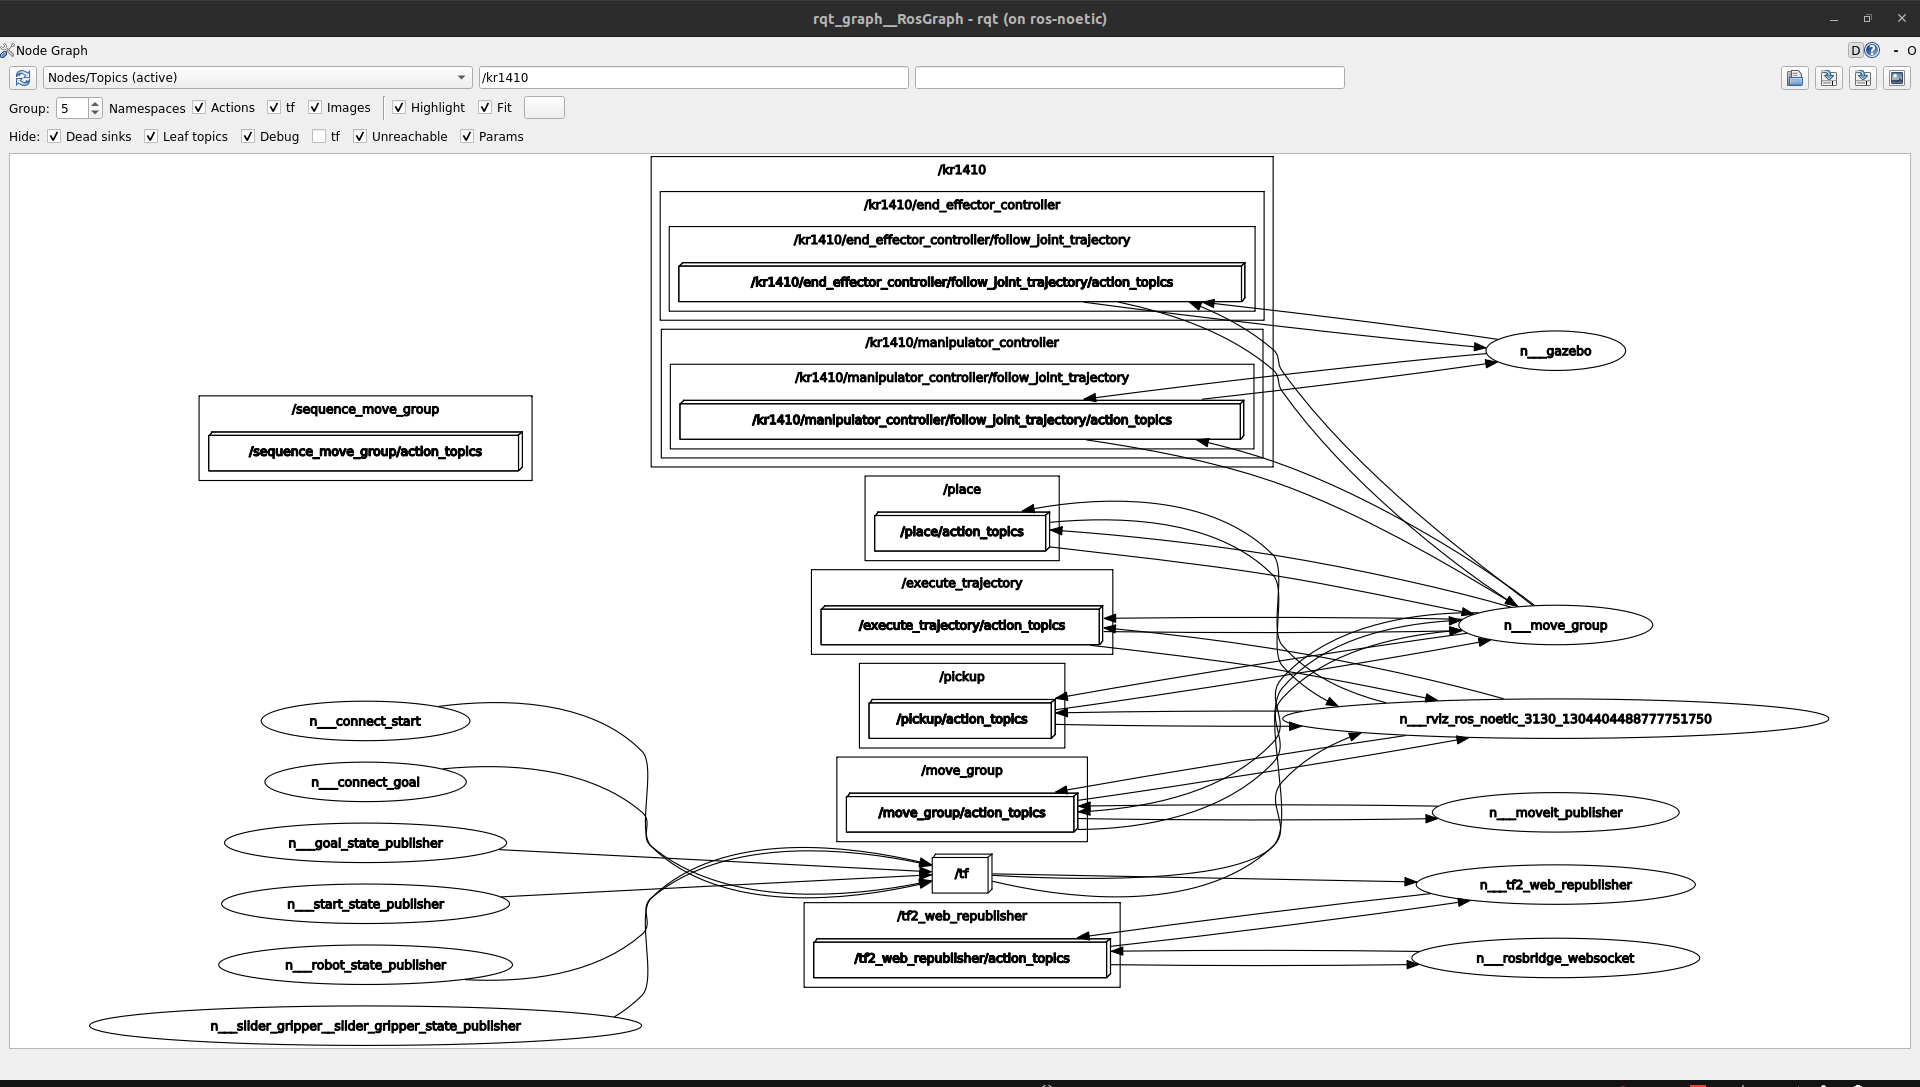
\includegraphics[width=\textwidth]{figures/rosgraph.png}
    \caption{ROSGraph}
    \label{fig:rosgraph}
\end{figure}

Many custom \hyperref[acro:ROS]{ROS} packages \cite{rospackage} are created to simulate the workcell. A single \hyperref[acro:ROS]{ROS} launch \cite{roslaunch} file is launched to run every node \cite{rosnode}, service \cite{rosservice} and parameter \cite{parameterserver} or action servers \cite{actionserver}
Figure \ref{fig:rosgraph} visualizes the computation graph of the simulation. It shows the currently active \hyperref[acro:ROS]{ROS} nodes \cite{rosnode}
and topics \cite{rostopic} in the simulation of robotic workcell.


\subsubsection{Gazebo Simulator}
\label{subsubsec:gazebo}
Gazebo is a \hyperref[acro:3D]{3D} dynamic simulator with the ability to accurately and efficiently simulate populations
of robots in complex indoor and outdoor environments. While similar to game engines, Gazebo
offers physics simulation at a much higher degree of fidelity, a suite of sensors, and interfaces for
both users and programs. \cite{gazebo-classic}

A model of the entire workcell is created for the gazebo simulator. The assets are converted from \hyperref[acro:CAD]{CAD} designs
to \textit{.dae} and \textit{.stl} file format using blender software. These meshes are then included in the SDF model object.
The workcell is then ready to be simulated in the gazebo simulator.

\begin{figure}[h]
    \centering
    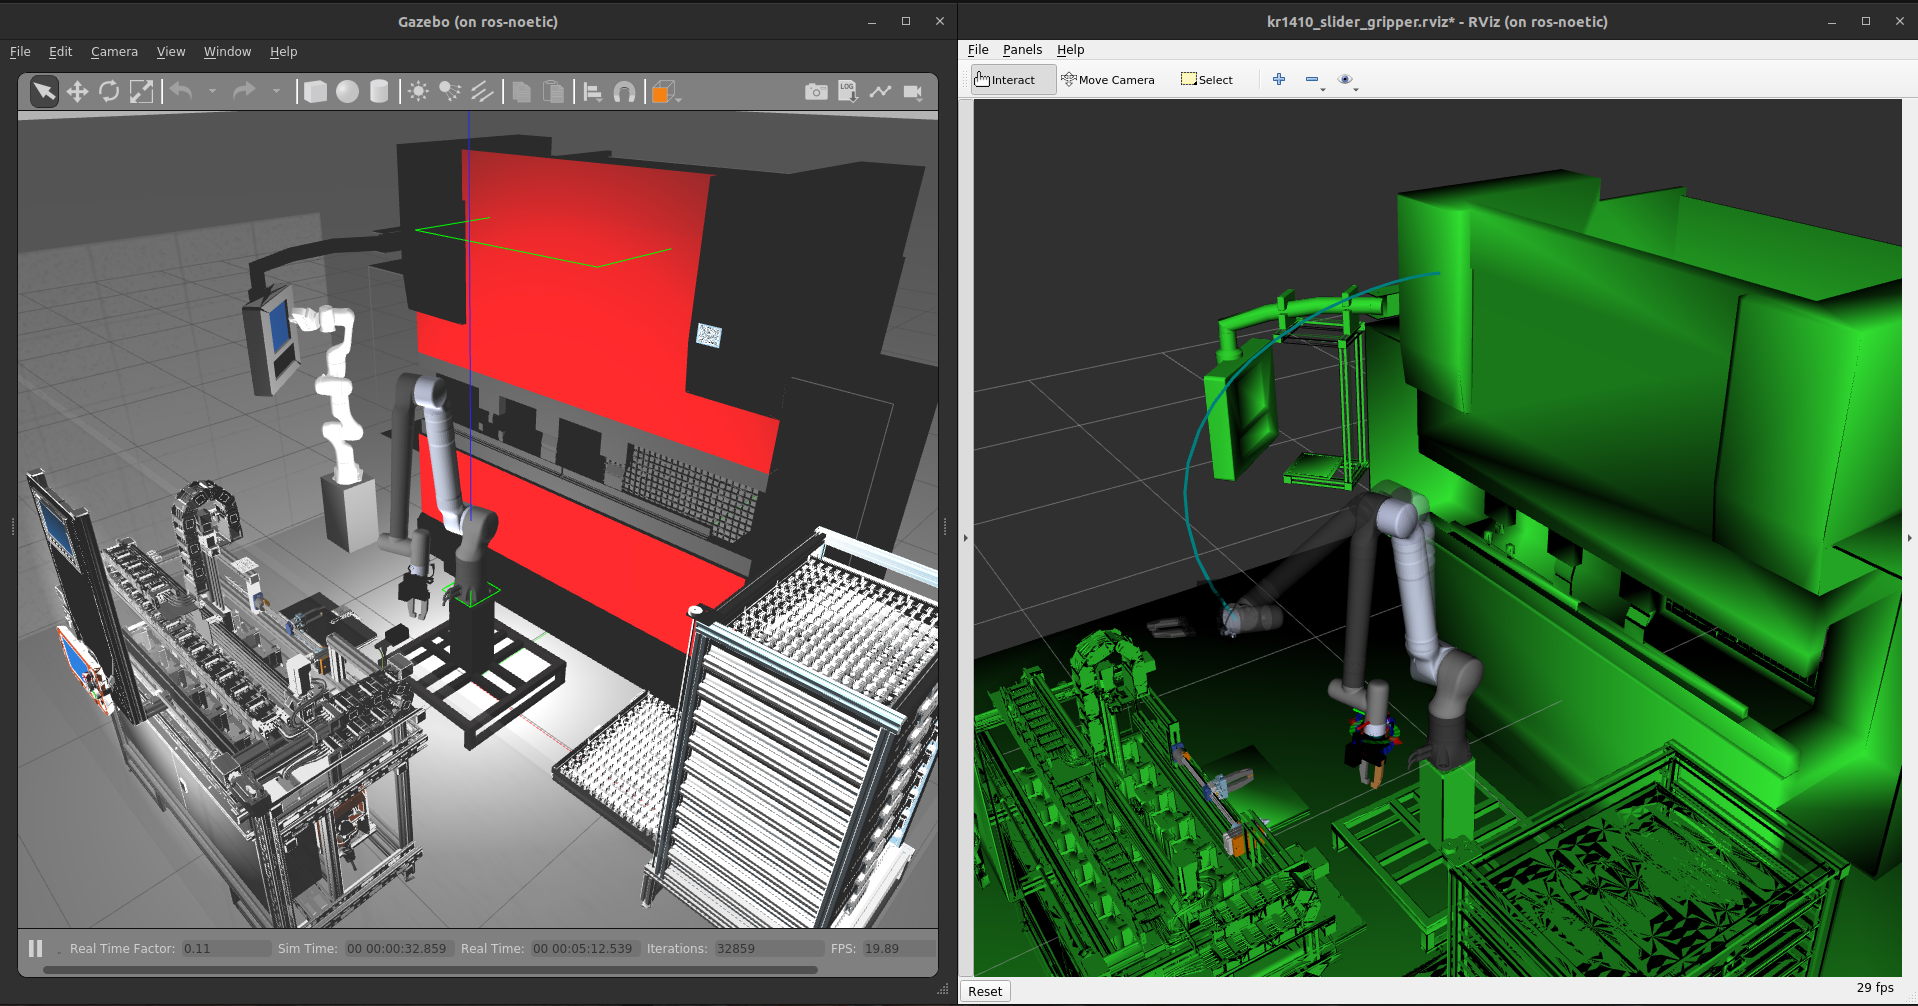
\includegraphics[width=\textwidth]{figures/gazebo-rviz.png}
    \caption{Robotic workcell in Gazebo simulator (left) and RViz (right)}
    \label{fig:gazebo-rviz}
\end{figure}

\subsubsection{RViz}
\label{subsubsec:RViz}
RViz is short for ROS Visualization. It is a \hyperref[acro:3D]{3D} visualization software tool for robots, sensors, and algorithms.
It allows seeing the robot's perception of its world (real or simulated).
The purpose of RViz is to visualize the state of a robot. It uses sensor data to try
to create an accurate depiction of what is going on in the robot's environment. \cite{rviz}

\subsubsection{MoveIt}
\label{subsubsec:moveit}
MoveIt is a software for \hyperref[acro:ROS]{ROS} used for manipulation, motion planning, \hyperref[acro:3D]{3D} perception, kinematics, control and navigation. \cite{moveit}
MoveIt is used to get to solve the kinematics of the 7-axis Kassow robot and do robotic manipulation and perception.
A collision mesh of the workcell is published in the planning scene as can be seen in RViz in Figure \ref{fig:gazebo-rviz}.
This makes the \hyperref[acro:KR]{KR1410} to plan trajectories without any collision in the workcell. The robotic gripper is also controlled using MoveIt package.
